\subsection{Real-data stopping results (P5)}
\label{sec:backtest}
The completed frozen grid contains 3,348 method evaluations: 31 market folds,
three seeds, two objectives, three cost scenarios and six methods. The runner
reports zero failed or pending evaluations and matching support. Real E5 uses
the P4 preparation and evaluation harness; older synthetic E5 files in
\texttt{results/paths/} are excluded.

\paragraph{Estimands and uncertainty.}
The tables report window-weighted mean scores, averaging seeds within each
window. Linear reward equals economic net return. Exponential reward is
\[u(r)=(1-\exp(-5r))/5.\]
Utility scores are not percentage returns and must not be
compared numerically with linear scores. The primary contrast is GRU minus MLP;
secondary contrasts compare GRU with LSM, Hold, TakeProfitStopLoss and
TrailingStop. Positive differences favor GRU.
The generated table gives 95\% paired moving-block intervals with 30-calendar-day
blocks, all assets on a date together, and separate resampling within folds.
The JSON artifact also contains 15/60-day sensitivity and per-seed estimates.
Two-sided null-centered bootstrap p-values use 2,000 replicates and seed zero
(the manifest records the actual count for regeneration).
Holm correction applies separately to the configured primary and secondary
families within each market, objective, cost and metric; it does not control
error across all reported scenarios. Cost and calendar-slice means are descriptive.

\begin{center}\scriptsize
\resizebox{\linewidth}{!}{\begin{tabular}{lllrrrr}
\toprule
market & objective & metric & estimate & ci\_lower & ci\_upper & p\_value\_holm \\
\midrule
nifty50 & linear & objective & -0.000835 & -0.002776 & 0.002218 & 0.577711 \\
nifty50 & linear & net\_return & -0.000835 & -0.002776 & 0.002218 & 0.577711 \\
nifty50 & exponential & objective & 0.000535 & -0.002275 & 0.004276 & 0.754123 \\
nifty50 & exponential & net\_return & 0.000138 & -0.001702 & 0.002302 & 0.880560 \\
sp100 & linear & objective & 0.000879 & -0.001068 & 0.003309 & 0.574213 \\
sp100 & linear & net\_return & 0.000879 & -0.001068 & 0.003309 & 0.574213 \\
sp100 & exponential & objective & 0.004224 & 0.000417 & 0.007249 & 0.017991 \\
sp100 & exponential & net\_return & 0.002699 & 0.000002 & 0.005153 & 0.044978 \\
crypto & linear & objective & -0.001627 & -0.013100 & 0.004869 & 0.750625 \\
crypto & linear & net\_return & -0.001627 & -0.013100 & 0.004869 & 0.750625 \\
crypto & exponential & objective & 0.000373 & -0.002497 & 0.004021 & 0.829585 \\
crypto & exponential & net\_return & -0.000378 & -0.001938 & 0.002530 & 0.768116 \\
\bottomrule
\end{tabular}
}
\end{center}
nifty50 under linear training: GRU has lower mean objective score than MLP; the interval includes zero.

nifty50 under linear training: GRU has lower mean economic net return than MLP; the interval includes zero.

nifty50 under exponential training: GRU has higher mean objective score than MLP; the interval includes zero.

nifty50 under exponential training: GRU has higher mean economic net return than MLP; the interval includes zero.

sp100 under linear training: GRU has higher mean objective score than MLP; the interval includes zero.

sp100 under linear training: GRU has higher mean economic net return than MLP; the interval includes zero.

sp100 under exponential training: GRU has higher mean objective score than MLP; the interval excludes zero.

sp100 under exponential training: GRU has higher mean economic net return than MLP; the interval excludes zero.

crypto under linear training: GRU has lower mean objective score than MLP; the interval includes zero.

crypto under linear training: GRU has lower mean economic net return than MLP; the interval includes zero.

crypto under exponential training: GRU has higher mean objective score than MLP; the interval includes zero.

crypto under exponential training: GRU has lower mean economic net return than MLP; the interval includes zero.

\paragraph{Costs and regimes.}
Every 0x, 1x and 2x scenario rebuilds reward and refits learned methods.
The venue-specific base fees, spread, slippage and funding assumptions are
recorded in the frozen config and each resolved scenario config.
\texttt{market\_cost\_tables.csv} separates utility and economic returns;
\texttt{regime\_tables.csv} provides 2020, 2022 and other-year slices and support
counts. These are descriptive calendar periods, not validated calm/stress
classifications. The available data do not cover 2008. Task 5's broader regime
and Hurst diagnostics remain outstanding.
\begin{center}\scriptsize
\resizebox{.85\linewidth}{!}{\begin{tabular}{llrrrr}
\toprule
market & objective & cost & OSPG-GRU & OSPG-MLP & GRU minus MLP \\
\midrule
crypto & exponential & 0 & 0.0019 & 0.0018 & 0.0001 \\
crypto & exponential & 1 & 0.0003 & 0.0006 & -0.0004 \\
crypto & exponential & 2 & -0.0035 & -0.0024 & -0.0011 \\
crypto & linear & 0 & 0.0367 & 0.0379 & -0.0012 \\
crypto & linear & 1 & 0.0331 & 0.0348 & -0.0016 \\
crypto & linear & 2 & 0.0299 & 0.0323 & -0.0024 \\
nifty50 & exponential & 0 & 0.0086 & 0.0071 & 0.0014 \\
nifty50 & exponential & 1 & 0.0047 & 0.0046 & 0.0001 \\
nifty50 & exponential & 2 & 0.0010 & 0.0022 & -0.0011 \\
nifty50 & linear & 0 & 0.0161 & 0.0148 & 0.0013 \\
nifty50 & linear & 1 & 0.0117 & 0.0126 & -0.0008 \\
nifty50 & linear & 2 & 0.0090 & 0.0095 & -0.0005 \\
sp100 & exponential & 0 & 0.0043 & 0.0024 & 0.0020 \\
sp100 & exponential & 1 & 0.0041 & 0.0014 & 0.0027 \\
sp100 & exponential & 2 & 0.0030 & 0.0012 & 0.0018 \\
sp100 & linear & 0 & 0.0079 & 0.0073 & 0.0006 \\
sp100 & linear & 1 & 0.0075 & 0.0067 & 0.0009 \\
sp100 & linear & 2 & 0.0070 & 0.0062 & 0.0007 \\
\bottomrule
\end{tabular}
}
\end{center}
\begin{center}\scriptsize
\resizebox{.85\linewidth}{!}{\begin{tabular}{lllrrr}
\toprule
market & objective & regime & OSPG-GRU & OSPG-MLP & GRU minus MLP \\
\midrule
crypto & exponential & 2022 & -0.0035 & -0.0035 & 0.0000 \\
crypto & exponential & other years & 0.0018 & 0.0024 & -0.0005 \\
crypto & linear & 2022 & -0.0486 & -0.0366 & -0.0119 \\
crypto & linear & other years & 0.0666 & 0.0640 & 0.0026 \\
nifty50 & exponential & 2020 & 0.0162 & 0.0158 & 0.0004 \\
nifty50 & exponential & 2022 & -0.0022 & -0.0018 & -0.0004 \\
nifty50 & exponential & other years & 0.0035 & 0.0033 & 0.0002 \\
nifty50 & linear & 2020 & 0.0165 & 0.0284 & -0.0119 \\
nifty50 & linear & 2022 & 0.0001 & 0.0018 & -0.0017 \\
nifty50 & linear & other years & 0.0136 & 0.0112 & 0.0024 \\
sp100 & exponential & 2020 & 0.0215 & 0.0136 & 0.0080 \\
sp100 & exponential & 2022 & -0.0017 & -0.0098 & 0.0081 \\
sp100 & exponential & other years & 0.0011 & 0.0011 & -0.0000 \\
sp100 & linear & 2020 & 0.0187 & 0.0265 & -0.0078 \\
sp100 & linear & 2022 & -0.0099 & -0.0086 & -0.0013 \\
sp100 & linear & other years & 0.0091 & 0.0054 & 0.0037 \\
\bottomrule
\end{tabular}
}
\end{center}

\paragraph{Memory diagnostic.}
The persistence plot uses lag-one absolute-log-return autocorrelation estimated
only before each fold's validation start, against the asset/fold GRU-minus-MLP
economic return at base costs. Points reuse assets across folds and are dependent;
the plot is exploratory and does not establish causation or long memory.
\begin{center}
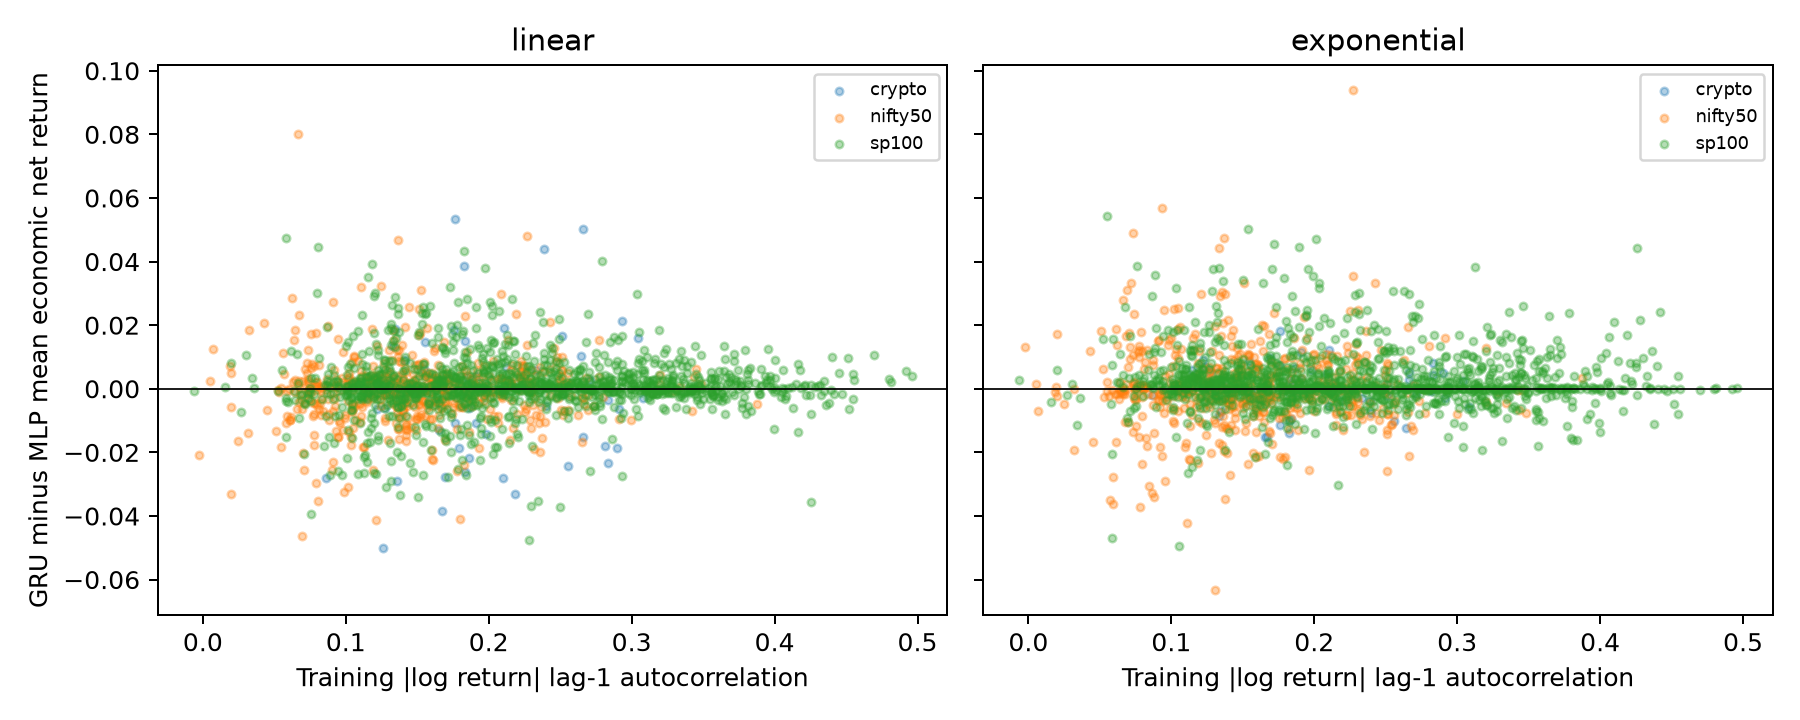
\includegraphics[width=.95\linewidth]{../results/p5/summary/persistence.png}
\end{center}

\paragraph{Validity and interpretation.}
The evaluation checks prefix causality, finite outputs, matched test windows,
scheduled-deadline purging before validation and test boundaries, and exits
within each window's terminal index. No extra embargo is added beyond that
purge. Learned methods use a global entry-day decision; immediate-exit rates
are retained in fold status files. These checks do not eliminate all model risk.
Current/retrieval-date universes induce survivorship and selection bias.
Adjusted daily-close execution and proportional costs are stylized; an order
submitted after observing a close is not assured that fill. Overlapping trade
windows do not constitute a self-financing portfolio or an annualized return.

The optional stopping theorem does not promise trading profits: under its
conditions, stopping an appropriate martingale preserves its expectation.
These physical-market, cost-adjusted payoffs need not be martingales. Differences
between fitted policies assess this experimental stopping problem and do not
disprove optional stopping or establish arbitrage. Concave utility can change
policy rankings by penalizing losses; compare the two objectives on economic
returns as well as on their own utility, using the intervals rather than signs alone.
All numbers and the plot trace to the summary script and its SHA-256 manifest.
P4 methodology review is pending.
